\documentclass[journal,12pt,twocolumn]{IEEEtran}

\usepackage{graphicx}
\graphicspath{ {./5600/} }
\usepackage{amsmath}
\newcommand{\myvec}[1]{\ensuremath{\begin{pmatrix}#1\end{pmatrix}}}
\title{ Assignment1}
\author{PARIMISETTY HARINADHA (CS19RESCH11004)}
\begin{document}
\maketitle
\newpage
\begin{abstract}
This document explains the concept of collinear and whether the triangle formed by given 3 points is right angled triangle or not.
\end{abstract}
Download all python codes from 
\framebox[1\width]{ https://github.com/cs19resch11004/5600/hari }
Download all Latex-tikz codes from 
\framebox[1.1\width]{ https://github.com/cs19resch11004/5600/hari} 
\section{Problem}
Without using the Pythagoras theorem, show that \myvec{ 4 \\ 4 }, \myvec{ 3 \\ 5 } and \myvec{ -1 \\ -1 } are the vertices of a right angled triangle?
\section{Explanation}
Initially we will test whether given 3 points are collinear or not. If they are non-collinear then we will check whether the triangle formed by given 3 points is right angled triangle or not by using one of the follwing 2 methods.
1. Direction vector based method
2. Slope method
In this document we are going to use Direction vector based method.\\
	Let A, B and C are 3 non-collinear points, then we will test, whether any two of the following Direction vectors A-B and A-C or A-B and B-C or A-C and B-C are perpendicular to each other or not by using DOT PRODUCT.
\section{Solution}
The direction vectors of A-B, A-C and B-C are
\begin{align}
	A-B=\myvec{-1 \\ 1} \\
	A-C=\myvec{-5 \\ -5}\\
	B-C=\myvec{-4 \\ -6} 
\end{align}
\begin{enumerate}
\item Testing of  A-B and B-C are perpendicular to each other or not?
DOT PRODUCT of  A-B and B-C is, \begin{align} \myvec{ -1 & 1 } . \myvec{ -4 \\ -6 } = -2\end{align}\\
A-B . B-C = -2 $\neq$ 0
Sides AB and BC of triangle are not perpendicular.


\item Testing of  A-C and B-C are perpendicular to each other or not?\\
DOT PRODUCT of  A-C and B-C is, \begin{align} \myvec{ -5 & -5 } . \myvec{ -4 \\ -6 } = 50\end{align}\\
A-C . B-C = 50 $\neq$ 0 
Sides AC and BC of triangle are not perpendicular.


\item Testing of  A-B and A-C are perpendicular to each other or not?\\
DOT PRODUCT of  A-B and A-C is, \begin{align} \myvec{ -1 & 1 } . \myvec{ -5 \\ -5 } = 0\end{align}\\
A-B . A-C, which is 0 
Sides AB and AC of triangle are perpendicular to each other. So Triangle ABC is right angled triangle and right angle at vertex \myvec{ 4 \\ 4 }, and the following figure represents the triangle formed by given points A, B and C.  
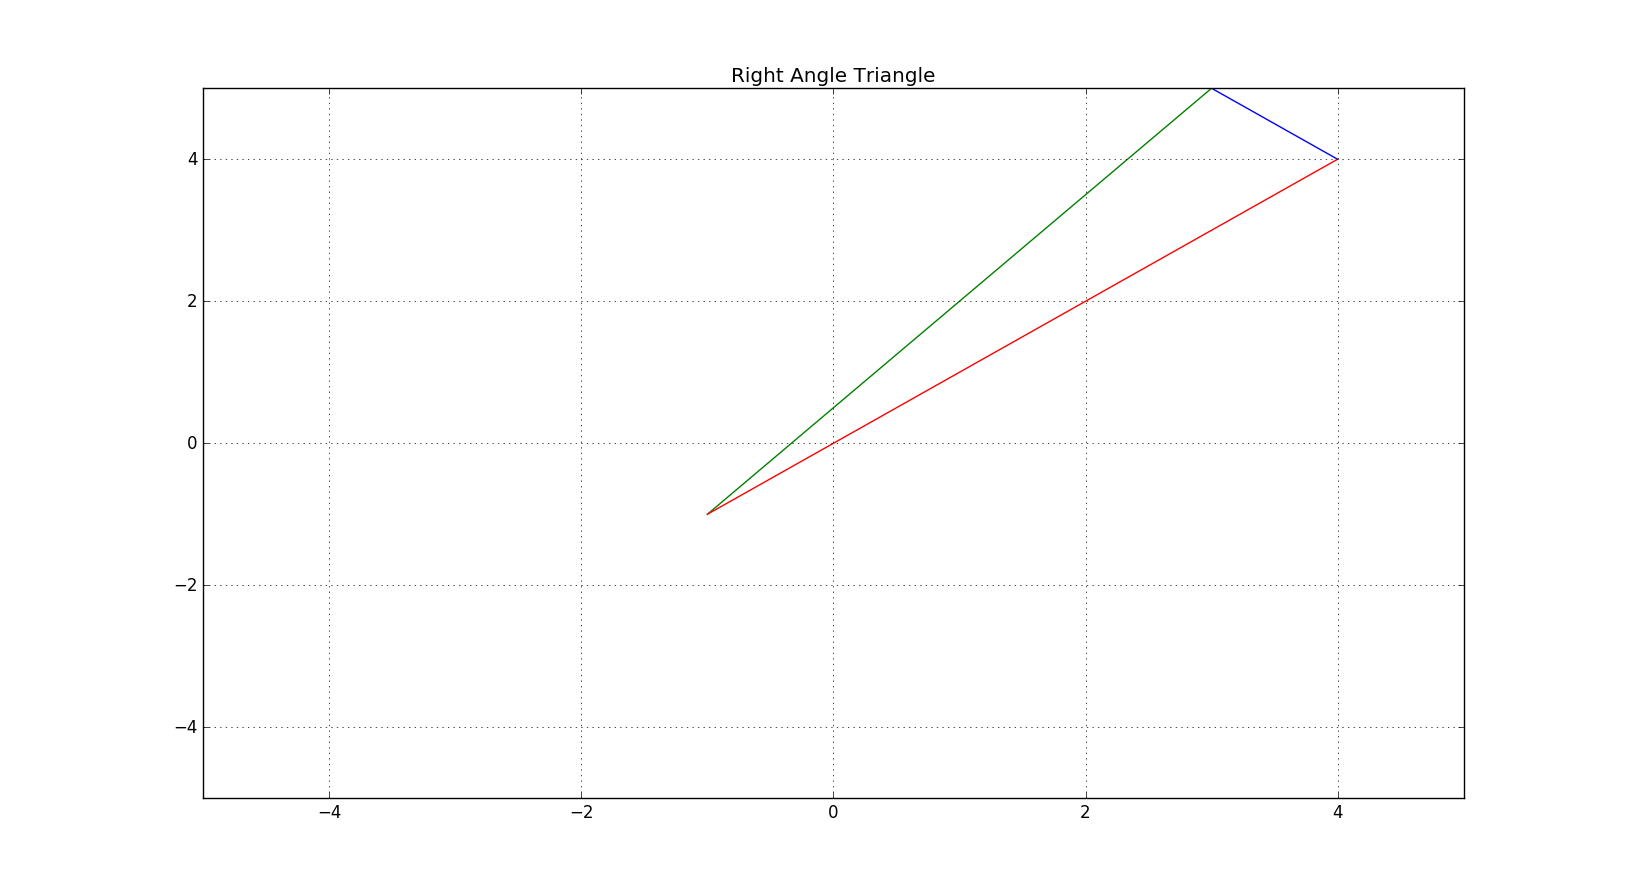
\includegraphics[width=15cm, height=10cm]{vihi}
\end{enumerate}
\end{document}
